% What abliteration actually changes inside a transformer block.
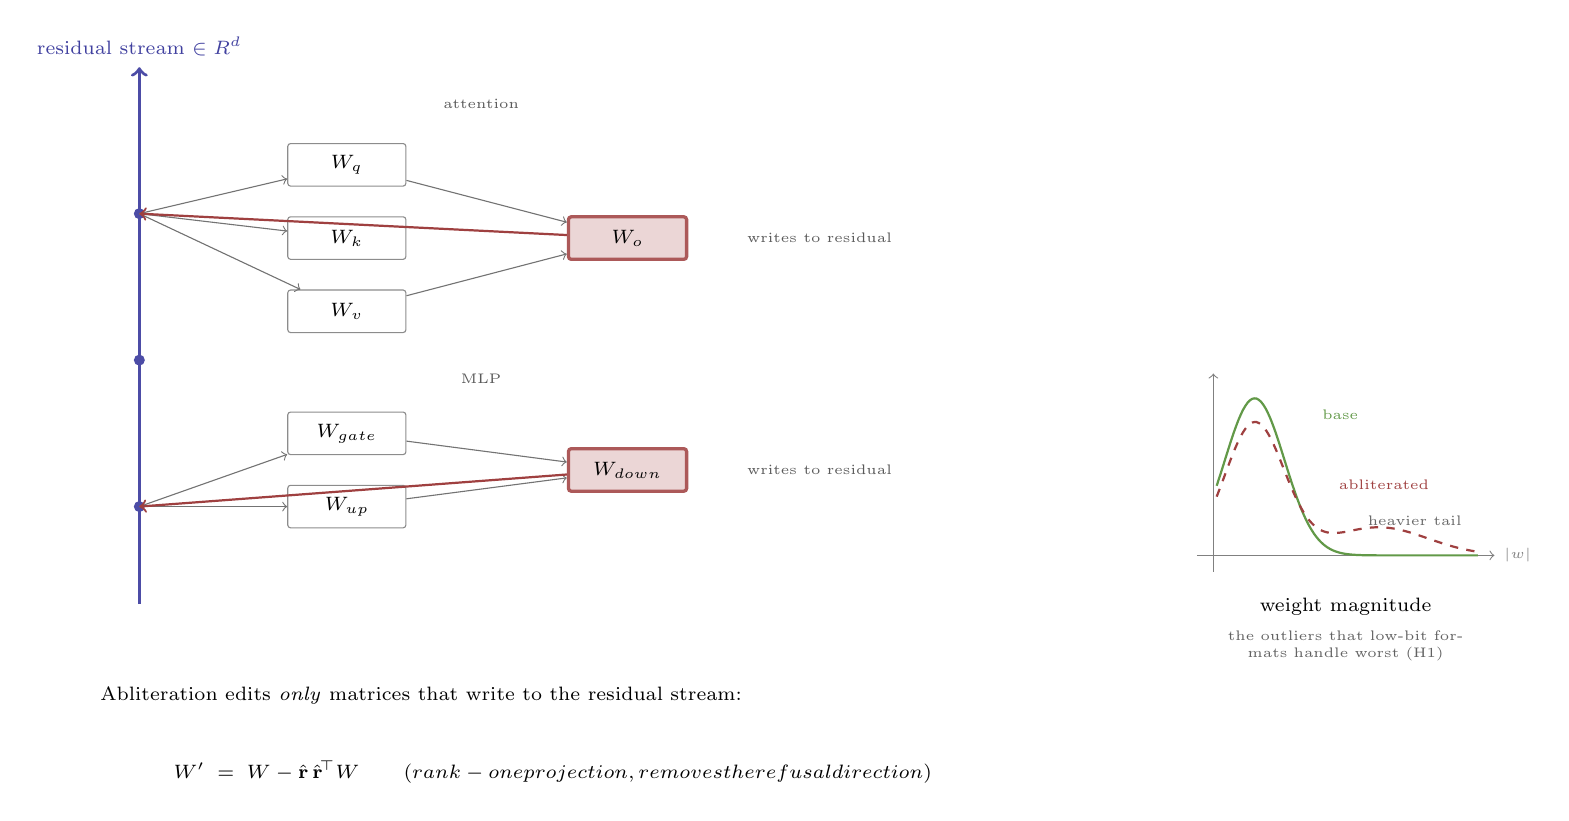
\begin{tikzpicture}[
  font=\scriptsize, x=1.55mm, y=1.55mm, node distance=0mm,
  blk/.style={draw=black!45, rounded corners=1pt, minimum width=15mm,
              minimum height=5.4mm, inner sep=1pt, fill=white},
  edited/.style={blk, fill=Maroon!16, draw=Maroon!65, very thick},
  res/.style={draw=NavyBlue!70, very thick},
  lab/.style={font=\tiny, text=black!65},
]
% residual stream
\draw[res, ->] (0,0) -- (0,44) node[above, font=\scriptsize, text=NavyBlue!75]
  {residual stream $\in\mathbb{R}^{d}$};
\foreach \y in {8,20,32} \fill[NavyBlue!70] (0,\y) circle (0.7mm);

% attention block
\node[blk] (q) at (17,36) {$W_q$};
\node[blk] (k) at (17,30) {$W_k$};
\node[blk] (v) at (17,24) {$W_v$};
\node[edited] (o) at (40,30) {$W_o$};
\node[lab, anchor=west] at (49,30) {writes to residual};
\draw[->, black!55] (0,32) -- (q); \draw[->, black!55] (0,32) -- (k);
\draw[->, black!55] (0,32) -- (v);
\draw[->, black!55] (q) -- (o); \draw[->, black!55] (v) -- (o);
\draw[->, Maroon!75, thick] (o) -- (0,32);
\node[lab] at (28,41) {attention};

% MLP block
\node[blk] (g) at (17,14) {$W_{\text{gate}}$};
\node[blk] (u) at (17,8) {$W_{\text{up}}$};
\node[edited] (d) at (40,11) {$W_{\text{down}}$};
\node[lab, anchor=west] at (49,11) {writes to residual};
\draw[->, black!55] (0,8) -- (g); \draw[->, black!55] (0,8) -- (u);
\draw[->, black!55] (g) -- (d); \draw[->, black!55] (u) -- (d);
\draw[->, Maroon!75, thick] (d) -- (0,8);
\node[lab] at (28,18.5) {MLP};

% the edit
\node[anchor=north west, font=\scriptsize] at (-4,-6)
  {Abliteration edits \emph{only} matrices that write to the residual stream:};
\node[anchor=north west] at (2,-12)
  {$W' \;=\; W - \hat{\mathbf r}\,\hat{\mathbf r}^{\!\top} W
    \qquad\text{(rank-one projection, removes the refusal direction)}$};

% distribution shift
\begin{scope}[shift={(88,4)}, x=1.05mm, y=1.05mm]
  \draw[->, black!50] (-2,0) -- (34,0) node[right, font=\tiny] {$|w|$};
  \draw[->, black!50] (0,-2) -- (0,22);
  \draw[OliveGreen!75, thick, smooth, samples=60, domain=0.4:32]
    plot (\x, {19*exp(-((\x-5)^2)/26)});
  \draw[Maroon!75, thick, dashed, smooth, samples=60, domain=0.4:32]
    plot (\x, {16*exp(-((\x-5)^2)/26) + 3.4*exp(-((\x-20)^2)/70)});
  \node[font=\tiny, text=OliveGreen!75, anchor=west] at (12,17) {base};
  \node[font=\tiny, text=Maroon!75, anchor=west] at (14,8.5) {abliterated};
  \node[font=\tiny, text=black!60, anchor=west] at (17.5,4.2) {heavier tail};
  \node[font=\scriptsize, anchor=north] at (16,-4) {weight magnitude};
  \node[font=\tiny, text=black!62, anchor=north, text width=42mm, align=center]
    at (16,-8) {the outliers that low-bit formats handle worst (H1)};
\end{scope}
\end{tikzpicture}
